\chapter{Porównanie i analiza aplikacji}
\label{roz7}
%=================================================================================================
Poprzednie rozdziały przedstawiły proces tworzenia~i wdrażania aplikacji monolitycznej, a także jej odpowiednika opartego~o mikrousługi. Po opracowaniu środowiska produkcyjnego możliwe jest przeprowadzenie badań mających na celu porównanie obu tych systemów. Istotne~w nich będą takie parametry jak wydajność, skalowalność~i łatwość implementacji.

\section{Cel~i zakres badań}
Celem badań jest przeprowadzenie porównania wydajności obu serwisów~w środowiskach produkcyjnych. Przebadane zostanie to jak podział aplikacji na mniejsze usługi wpływa na ogólną sprawność serwisu~w porównaniu do jednej scentralizowanej aplikacji. Następnie sprawdzone zostanie, jak zmieniają się osiągi aplikacji przy ich skalowaniu, czyli zwiększaniu ilości zasobów sprzętowych~i liczby kontenerów, które mogą obsługiwać żądania. Analizie zostanie poddana implementacja poszczególnych serwisów, tak, aby porównać otrzymane wyniki do zastosowanych technologii, skali projektu, trudności~w przygotowaniu architektury~i zastosowania danych rozwiązań technologicznych. Celem badań jest wskazanie podobieństw~i właściwości poszczególnych podejść. Znalezienie ich atutów~i wad, a następnie wskazanie przypadków, gdzie wykorzystanie danej architektury byłoby korzystniejsze.

Do testów wydajności wykorzystane będzie narzędzie \textit{Boom}. Jest to biblioteka napisana~w języku Python przez autora książki \textit{Rozwijanie mikrousług~w Pythonie}\cite{Ziade:2018}, której zadaniem jest przeprowadzenie testów obciążeniowych serwera. Przesyła ona do niego zadaną ilość żądań symulując ruch~w danym serwisie, a następnie dla każdego~z nich mierzy czas. Wyniki tych operacji uśrednia podając całkowity czas przeprowadzonego testu, najszybciej~i najdłużej wykonane żądanie, a także ich średni czas, amplitudę, ilość żądań na sekundę.
\newpage
\begin{lstlisting}[language=Bash, caption={Przykładowy test przy wykorzystaniu narzędzia \textit{Boom}.}]
$user@home: boom http://localhost:80 -c 10 -n 100
Server Software: nginx/1.17.10
Running GET http://127.0.0.1:80
	Host: localhost
Running 100 queries - concurrency 10
[=================================================================>] 100% Done

-------- Results --------
Successful calls		100
Total time        		0.8767 s
Average           		0.0839 s
Fastest           		0.0317 s
Slowest           		0.1165 s
Amplitude         		0.0848 s
Standard deviation		0.016234
RPS               		114
BSI              		Pretty good

-------- Status codes --------
Code 200          		100 times.

-------- Legend --------
RPS: Request Per Second
BSI: Boom Speed Index
\end{lstlisting}

Natomiast do przeprowadzenia analizy skalowalności również zostanie wykorzystane narzędzie \textit{Boom}, aby porównać jak zwiększenie ilości serwisów wpływa na wydajność aplikacji. Samo skalowanie aplikacji może zostać przeprowadzone przy wykorzystaniu platformy \textit{Docker}, posiada ona funkcję zwiększenia ilości zasobów takich jak ilość rdzeni, pamięci \textit{RAM}. Proces zmiany tych wartości nazywany jest \textit{skalowaniem~w pionie}\cite{Folwer:2019}.

Do \textit{skalowania~w poziomie}\cite{Folwer:2019} zostanie wykorzystana możliwość zwiększenia ilości kontenerów dla danego serwisu~w ramach narzędzia \textit{Docker Compose}. Przy pomocy polecenia \verb|docker-compose up --scale nazwa_serwisu=ilosc_kontenerow|, można przypisać ile kontenerów powinna mieć dana usługa~i dzięki temu zwiększyć przepustowość żądań aplikacji\cite{docker}.

W celach sprawdzenia łatwości implementacji danego rozwiązania przeprowadzone zostanie analiza poszczególnych fragmentów obu serwisów, ich rozbudowania, wymaganych zależności~i ocena zastosowanych rozwiązań architektonicznych.

\section{Wydajność}
W każdym badaniu przeprowadzonym przy pomocy programu \textit{Boom} wykorzystano takie same parametry, symulując ruch dla \textit{100} użytkowników, którzy wysyłają maksymalnie \textit{1000} żądań. Na początku przeprowadzono pomiar dla wszystkich dostępnych adresów~w obu serwisach. Aplikacja monolityczna obsługuje informację~o użytkowniku korzystając~z zmiennych globalnych, które są dostępne~w każdym~z widoków, dlatego nie potrzebuje ona zwracać informacji~o nim, w przeciwieństwie do aplikacji opartej~o mikrousługi, która na wykresie \ref{fig:microczasy} będzie miała, z tego powodu, jeden adres więcej. Dla zapytania \verb|\index| wyróżniono jeszcze przypadek, gdy użytkownik jest zalogowany (\textit{logged}). Wyniki przedstawiono na poniżej wykresach:
\begin{figure}[h!]
	\centering
		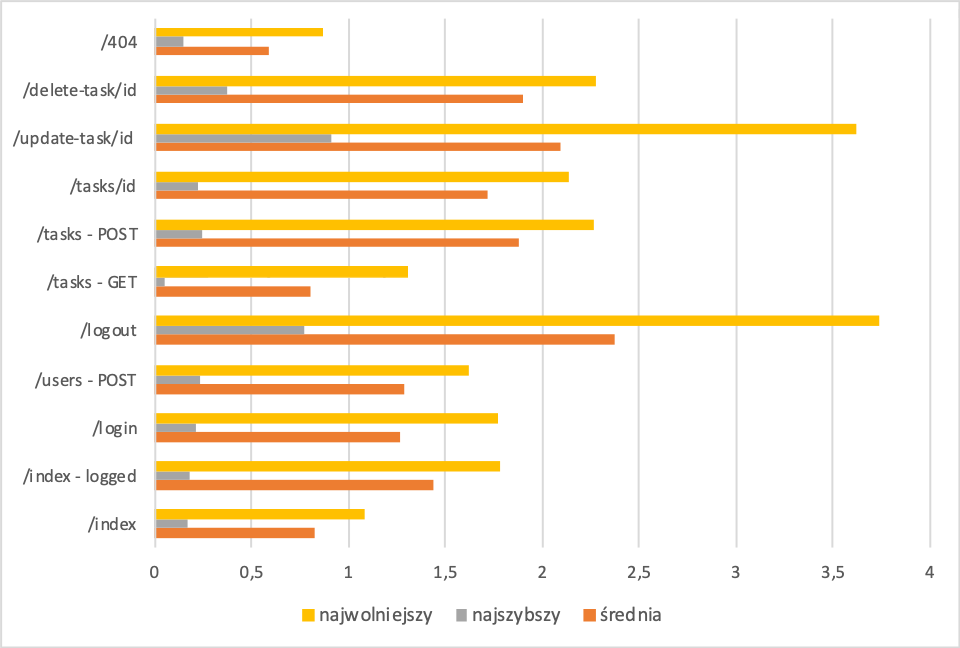
\includegraphics[width=12cm]{Rysunki/Rozdzial7/mono-zad.png}
		\caption{Czasy żądań (ms) dla każdego z adresu w aplikacji monolitycznej.}
		\label{fig:monoczasy}
	\end{figure}
\begin{figure}[h!]
	\centering
		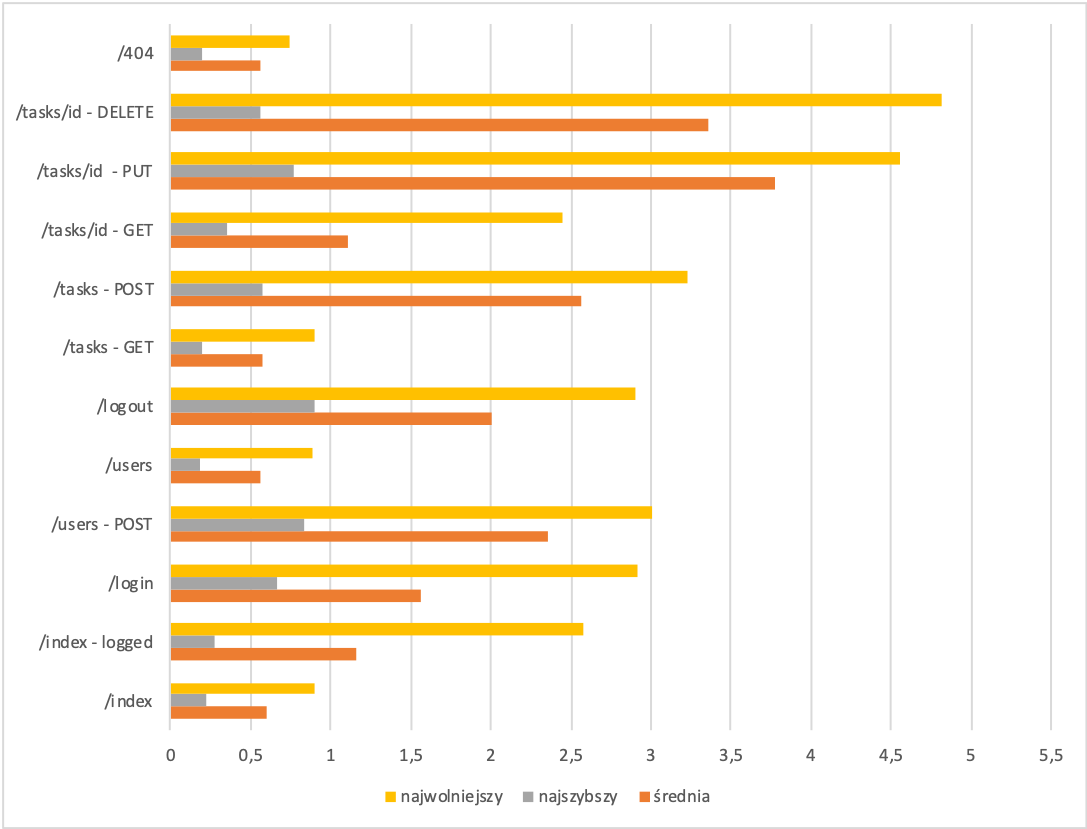
\includegraphics[width=12cm]{Rysunki/Rozdzial7/micro-zad.png}
		\caption{Czasy żądania (ms) dla każdego z adresu w aplikacji mikrousługowej.}
		\label{fig:microczasy}
	\end{figure}

Z wykresów (\ref{fig:microczasy}, \ref{fig:monoczasy}) wynika, że dla prostszych informacji do zwrócenia takich jak te~z adresów: \textit{index}, strona \textit{404}, obie aplikacje mają podobne wyniki~i zabierają im one najmniej czasu. Więcej zajmuje natomiast zwrócenie stron przy użyciu zapytania \textit{GET}, w tym przypadku widać, że nie ma reguły~i średni czas dla nich jest różny. Najdłużej~w aplikacji monolitycznej wykonywane są żądania odpowiadające za wylogowanie użytkownika, a także aktualizację zadania. Z kolei~w serwisie opartym~o mikrousługi najdłuższe jest usunięcie, a także jak~w przypadku pierwszej aplikacji zaktualizowanie zadania użytkownika.  Wynikać to może~z tego, że te żądania wymagają zweryfikowania wszystkich danych przesłanych~w zapytaniu, a następnie nadpisania lub usunięcia danego obiektu~z bazy danych.

Aplikacja oparta~o mikrousługi ma ogólnie gorsze średnie czasy~i dłuższe odpowiedzi, mimo, że dane zwracane przez serwer to proste obiekty \textit{JSON}, a nie całe struktury \textit{HTML} jak~w serwisie monolitycznym. Widocznie, przy niewielkich rozmiarach serwisów rodzaj przesyłanych danych nie wpływa na szybkość działania usług, a może go mieć ich \textit{serializacja} (mikrousługi) do formatu \textit{JSON}.

\section{Skalowalność}
W panelu ustawień platformy \textit{Docker} są funkcje odpowiedzialne za zarządzanie zasobami. Wśród nich możliwość zmiany ilości rdzeni procesora~i \textit{RAMu}, sterując tymi zależnościami zbadany będzie ich wpływ na szybkość zapytań.

\begin{figure}[h!]
	\centering
		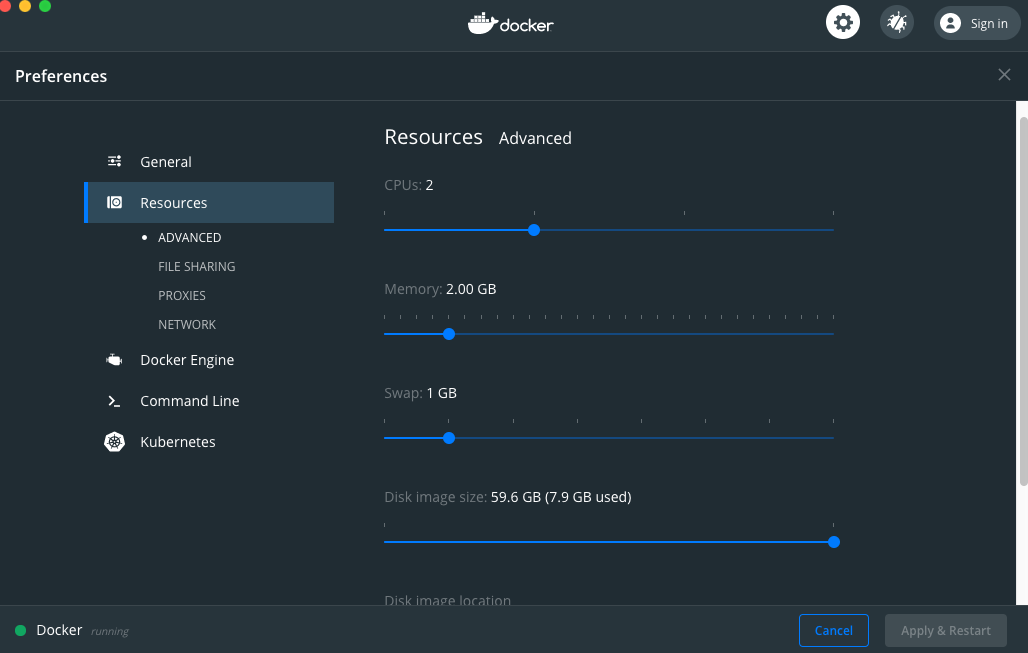
\includegraphics[width=12cm]{Rysunki/Rozdzial7/dockerpanel.png}
		\caption{Zakładka do zarządzania zasobami w ustawieniach platformy \textit{Docker}.}
		\label{fig:microczasy}
	\end{figure}
Badania obejmą sprawdzenie zmiany szybkości odpowiedzi serwera~w zależności od zasobów. Do ich przeprowadzania również wykorzystano narzędzie \textit{Boom}.

\begin{figure}[h!]
	\centering
		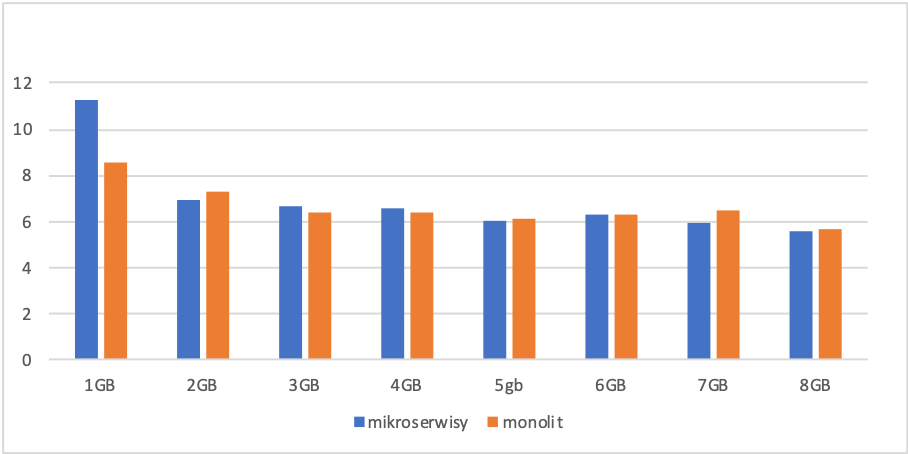
\includegraphics[width=12cm]{Rysunki/Rozdzial7/ramtest.png}
		\caption{Średnie czasy(ms) żądań w zależności od liczby posiadanej pamięci \textit{RAM}.}
		\label{fig:ramtest}
	\end{figure}
\begin{figure}[h!]
	\centering
		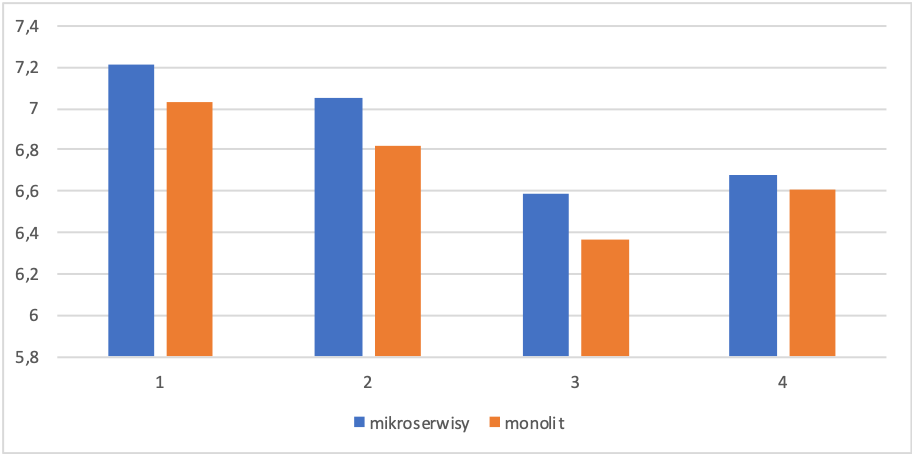
\includegraphics[width=12cm]{Rysunki/Rozdzial7/cputest.png}
		\caption{Średnie czasy żądania(ms) w zależności od liczby rdzeni w procesorze (\textit{CPU}).}
		\label{fig:cputest}
	\end{figure}
Na wykresie \ref{fig:ramtest} widać, że przy niewielkiej ilości pamięci \textit{RAM} ma on wpływ na działanie aplikacji szczególnie, gdy jest go niewiele, wówczas czasy żądań się wydłużają. Prawdopodobnie jest to związane~z tym, że serwisy wymagają minimalnej jego ilości do stabilnego działania, gdy ta zostanie osiągnięta to rola pamięci \textit{RAM} w szybkości obsługiwanych zapytań jest już mniej istotna~i czasy te pozostają na podobnym poziomie. 
Inną zależność można zauważyć~w przypadku liczby rdzeni na wykresie \ref{fig:cputest}, ich ilość nie wypływa na szybkość żądań, dopóki nie będzie ich więcej niż dwa. Każdy użytkownik to asynchroniczne zapytanie. W taki sposób program \textit{Boom} symuluje ruch na serwerze\cite{Ziade:2018}. Prawdopodobnie dwa rdzenie są wykorzystywane przez inne usługi~i zwiększenie ich ilości powoduje, że aplikacja lepiej sobie radzi~z obsługą zapytań, co może tłumaczyć spadek średniej czasów żądań przy trzech rdzeniach.

Następnym przeprowadzonym badaniem jest sprawdzenie skalowalności poziomej dla obu aplikacji, czyli tego jak zachowają się serwisy, gdy zwiększona będzie ilość ich instancji. \textit{Load balancer} zaimplementowany~w każdym~z nich powinien kierować ruchem tak, aby nie obciążać tylko jednego~z kontenerów, co powinno przyczynić się do szybszych czasów żądań\cite{Rodger:2019}.


\begin{figure}[h!]
	\centering
		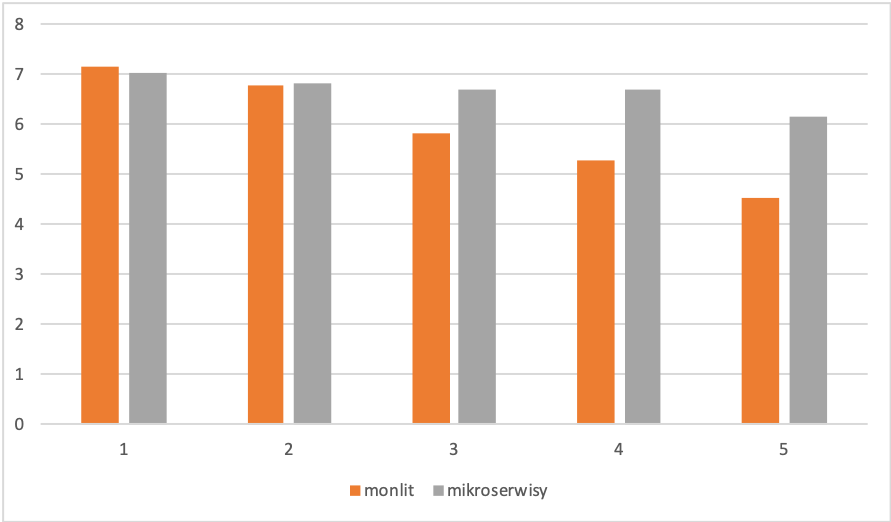
\includegraphics[width=12cm]{Rysunki/Rozdzial7/kontenery.png}
		\caption{Średnie czasy żądania(ms) w zależności od liczby powielonych kontenerów na jeden serwis.}
		\label{fig:kontenery}
	\end{figure}
	
W przypadku	badania skalowalności na wykresie \ref{fig:kontenery} widać tendencję spadkową, która jest zauważalnie większa przy aplikacji monolitycznej. Dla tego serwisu można również dostrzec, że przy liczbie kontenerów \textit{1}, radził on sobie nieznaczenie gorzej od mikroserwisów. Następnie dla dwóch kontenerów oba serwisy miały zbliżone czasy. Dopiero przy kolejnych pomiarach scentralizowana usługa uzyskała przewagę. Posiada ona jeden serwis napisany~w bibliotece \textit{Flask}, co sprawia, że ich skalowanie mniej obciąża maszynę. W aplikacji opartej~o mikrousługi potrzebne było stworzenie wielu instancji dla kilku usług, co~w ostateczności mogło mocniej obciążyć jednostkę, na której testowano serwisy~i zwiększyć czasy żądań aplikacji. 

Przeglądając otrzymane wyniki można zauważyć, że serwis mikrousługowy~w każdym~z porównań wypada gorzej, mimo, że to jego architektura zorientowana jest na łatwą skalowalność\cite{Rodger:2019}, to monolit wykorzystujący hierarchię klas do komunikacji, ma lepszą wydajność. Prawdopodobnie ilość potrzebnych serwisów~w aplikacji mikrousługowej jest niewspółmierna do obsługiwanych danych, rozmiarów projektu~i~w badanych warunkach zastosowane rozwiązania nie przynoszą żadnych dodatkowych korzyści~w polepszeniu wydajności aplikacji, a nawet wpływają na nią negatywnie.

\section{Analiza implementacji projektu}
Wskaźniki wydajności są istotne, ponieważ to one mogą być podstawą do rozważenia przejścia na daną architekturę. Inną decydującą cechą jest łatwość implementacji. To jakie rozwiązania należy zastosować, ich konfiguracja~i wykorzystywane technologie.

Aplikacja monolityczna głównie opiera się~o bibliotekę \textit{Flask} i proste szablony \textit{HTML}, których konfiguracja jest podstawowa. Wszystkie dodatkowe opcje, takie jak formularze są dostarczane przy pomocą zewnętrznego modułu \textit{Flask WTF}, a ich renderowanie odbywa się automatycznie przy pomocy metody \textit{render\_template}.
Do zarządzania sesją użytkownika również wykorzystywano dodatkową bibliotekę, która sprawia, że konfiguracja jest automatyczna, a dodatkowo wprowadza ona możliwość sprawdzenia danych klienta nawet~z szablonów, oferując globalny obiekt \textit{current\_user}. Nie jest potrzebne pobieranie danych~z bazy, a wylogowywanie użytkownika sprowadza się wyłącznie do wykorzystania funkcji \textit{logout\_user()}. 
Struktura projektu monolitycznego jest logiczna, wszystkie elementy aplikacji, które nie współgrają bezpośrednio są od siebie odseparowane, a konfiguracja aplikacji opiera się na przekazaniu niewielkiej ilości zmiennych globalnych~i podłączeniu~z bazą danych. Nie musi on być uruchamiany wewnątrz kontenera, aby komunikować się~z innymi komponentami, a projekt mógłby być bez problemu uruchomiony~i skonfigurowany nie wykorzystując platformy \textit{Docker}.

W przypadku aplikacji opartej na mikrousługach jej decentralizacja sprawia, że każdy~z serwisów jest osobno konfigurowany. Muszą one korzystać~z różnych bazy danych, co tworzy wiele utrudnień takich jak potrzeba powielania plików~z ustawieniami~i wielokrotne instalowania tych samych zależności. Struktura pomniejszych usług przypomina małą aplikację monolityczną, co sprawia, że~w każdej~z nich należy zaimplementować takie same mechanizmy obsługi żądań~i komunikacji~z usługą bazodanową. Zarządzenie sesjami użytkownika opiera się~o zewnętrzny mechanizm, z którym usługi muszą łączyć się przy pomocy protokołu \textit{HTTP} w celu autoryzacji. Baza danych tej usługi musi przechowywać wszystkie stworzone \textit{tokeny} i sprawdzać ich poprawność, co jest rozwiązaniem bardziej skomplikowanym niż zautomatyzowany proces uwierzytelniania~z aplikacji monolitycznej. Dodatkowo należy dbać~o integralność danych, sprawdzać~w każdej~z usług, nawet interfejsie użytkownika, czy żądanie posiada \textit{token}, a następnie przesyłać go dalej~w celu jego odszyfrowania.

Kilka baz danych to też problem~z ich zarządzaniem, potrzebne jest wdrażanie trzech osobnych migracji~i tworzenie tabel. Natomiast po stronie klienta, w przeglądarce internetowej potrzebne było wykorzystanie jej pamięci wewnętrznej (\textit{localStorage}) do przechowywania informacji~o użytkowniku~i wygenerowanych tokenów.

Interfejs użytkownika nie jest zbiorem kilku szablonów~w języku \textit{HTML}, ale osobną aplikacją zbudowaną przy pomocy programu generującego, który tworzy projekt~z wszystkimi strukturami~i konfiguracjami. Do swobodnego korzystania~z wszystkich bibliotek~w nim zawartych~i dowolnego ich konfigurowania, należy poznać wiele modułów frameworka \textit{Nuxt.js}. Są to znaczne ilości dodatkowych warstw abstrakcji~i ustawień~w projekcie.

Poszczególne aplikacje mogą działać osobno, ale tylko razem są możliwe do użytkowania, a do tego potrzebne jest stworzenie wielu plików konfiguracyjnych, niejednokrotnie~z powielonymi informacjami. Kontenery muszą wykorzystywać mechanizmy platformy \textit{Docker} do porozumiewania się, inaczej trzeba by było tworzyć fizyczne struktury sieciowe, a moduł do uwierzytelniania musiałby być widoczny jednie dla pozostałych serwisów wewnątrz prywatnej sieci, aby mógł bezpiecznie pobierać~i przekazywać dane.

Analizując oba podejścia widoczne jest, że aplikacja oparta~o mikroserwisy jest~o wiele trudniejsza do wdrożenia, czas jej stworzenia był dłuższy, wymagała ona skrupulatnego obmyślenia całej architektury, warstw komunikacji pomiędzy poszczególnymi elementami~i ręcznego wdrożenia wielu mechanizmów takich jak serializacja danych, proces uwierzytelniania użytkowników~i struktura zapytań serwera. Do jej szybkiej konfiguracji niezbędna jest platforma \textit{Docker}. Natomiast aplikacja monolityczna wszystkie te mechanizmy ma zaimplementowane~w ramach dodatkowych bibliotek frameworku \textit{Flask}, a sama struktura plików jest przejrzysta~i dobrze zorganizowana na warstwy logiczne, gdzie żadna~z nich się nie powiela.